%\chapter{State of the art}
\label{chap:chapter2}

% potentially make subsections;
% gamification
% stackoverflow as a platform
%etc
%\section[Stack Overflow]{\glsentrylong{so} (\glsentryshort{so})}
%\label{sec:stackoverflow}

\section[Stack Overflow]{\glsentrylong{so} (\glsentryshort{so})}
\label{sec:stackoverflow}

\subsection[Stack Overflows design]{\glsentrylong{so}s (\glsentryshort{so}) Design}
\label{sec:stackoverflow_design}
The following list shows the design used in \gls{so} (based on \textcite[p.~6-7]{M.Sewak2010} and \textcite[p.~805]{Treude2011}):
\begin{enumerate}
	\item Votes: Questions and answers which are considered good (or bad) by the community can be given a score. 
	This gives a filtering mechanisms, which allows users to ignore answers that are bad or wrong. 
	Furthermore, answers are sorted by votes, and you can also sort questions on \gls{so} by vote score 
	(see Figure \ref{fig:question_list_acc_answ}). 
	\item Accepted answer: If the user asking a question gets an answer that they find satisfactory, they can select it as the "accepted answer". 
	This answer will be the first displayed of the answers, and is also viewable when searching for questions 
	(see Figure \ref{fig:question_list_acc_answ} and \ref{fig:so_question_example}).
	\item Tags: Each question is associated with a tag\footnote{
		A full list can be seen here: \url{http://stackoverflow.com/tags/}
	}, which can be a topic, a programming language, a methodology, etc.
	\item Badges: Similar to achievements in games, Badges are used to reward the user for their participation.
	\item Reputation and Bounty: Currency system for user participation. 
	E.g. voting for questions, getting your answer selected as the accepted one, etc.
	Bounty is a trade, where if your question goes unanswered for too long, you offer up parts of your reputation to receive an answer.
	\item Data dump: Available data dump containing all content available within the \gls{se} community \cite{StackExchange2016}. 
	You can either download single files, or everything by using a Torrent client.
	\item Pre-Search: Encouraging users to check that their question is not already posted by presenting a search bar when asking a new question. 
	\item URL keywords and Google: The questions title is included in the URL, allowing it to be processed by search engines. 
	In addition, Google uses their crawlers every 10 second to have the latest updates from \glossary{so} in their search engine \cite{Gobry2011}.
	\item Critical mass: Before Atwood and Spoolsky launched \gls{so}, they invited developers and programmers to participate to have some domain experts available. 
\end{enumerate}

\clearpage
% figure showing questions, where one question has an accepted answer
\begin{figure}[ht]
	\centering
	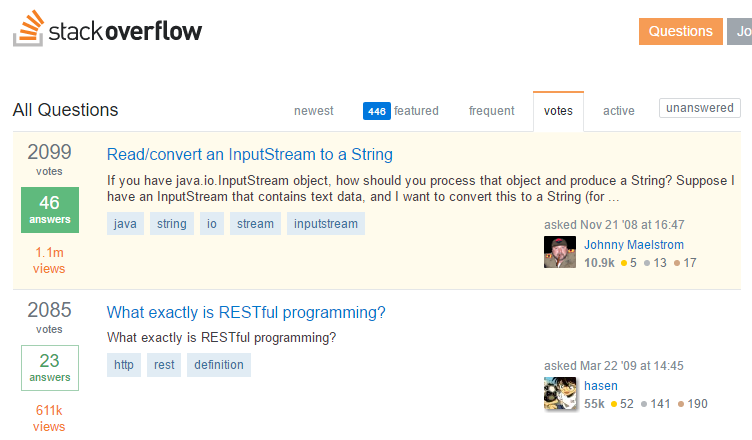
\includegraphics[width=0.5\textwidth]{question_list_acc_answ}
	\caption{List of questions, where one can see those with an accepted answers are marked with a green background.}
	\label{fig:question_list_acc_answ}
\end{figure}


% figure showing page with question and answer
\begin{figure}[ht]
	\centering
	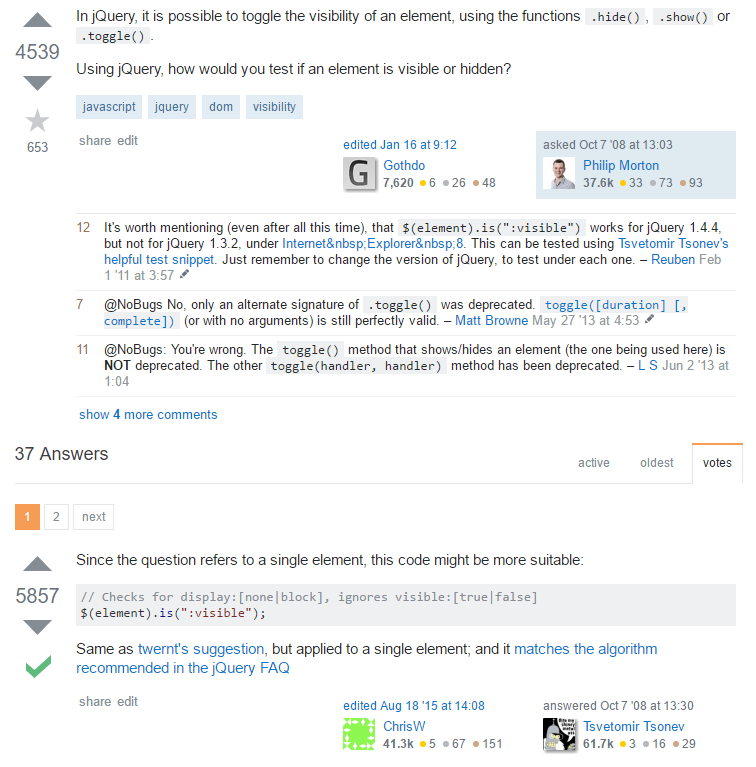
\includegraphics[width=0.5\textwidth]{so_question_example}
	\caption[Example of a question on Stack Overflow]{Example of a question on Stack Overflow\footnotemark}
	\label{fig:so_question_example}
\end{figure}
\footnotetext{Source: \url{http://stackoverflow.com/questions/178325/checking-if-an-element-is-hidden}}

\subsection[Stack Overflow and Gamification]{\glsentrylong{so} (\glsentryshort{so}) and Gamification}
\label{sec:stackoverflow_gamification}
\textcite{Deterding2011} defines Gamification as "the use of game design elements in non-game contexts", and is the definition this section will be based on. 
Several papers make notes of the pedagogical and educational aspect of \gls{so} \cite{Nasehi2012, Posnett2012, Yang2014}, and \cite{Nasehi2012, Yang2014} use the term gamification in their paper.
One of the founders, Jeff Atwood said in an interview that he wanted users to not just give good answers, but also trick them into improving their communication skills \cite{Posnett2012}\footnote{
	From this interview: \\ 
	\url{http://www.wired.com/2012/07/stackoverflow-jeff-atwood/2012}.
	}.
In the course IMT4007 Serious Games Simon McCallum and Marius Nowostawski, presented their game GoRad, which was based on us students reading articles and posting questions which were voted on. 
The \gls{so} system awards users based their activity by using votes, reputation and badges \cite{M.Sewak2010, Movshovitz-Attias2013, Treude2011, StackOverflow.com2016, StackOverflow.com2016d}.
In relation to gaming, there are four player types: Achievers, Explorers, Socializers and Killers \cite[p.~3]{Maan2013}.
\vspace{0.5em}\newline
These player types can be used as a representation\footnote{	
	\textcite{Yang2014} characterised users as "Sparrows" and "Owls", where sparrows answers question for reputation and owls answers the difficult ones (domain experts).  \\
	\textcite[p.~2]{Ahmed2015} defined users as "lurkers, help-seekers (askers) and givers (responders)".	
	} for the various users of \gls{so}. 
Achievers are there for the reputation and badges, socializers are to interact, discuss and share knowledge. 
Explorers might find joy in looking at various topics, or searching for unanswered questions.
The only exception would be the "Killer" type. 
Killers are those "\ldots who always want to create trouble/problems for other participants" \cite[p.~3]{Maan2013}. 
In an online \gls{qa} system (or Internet in general), these are what are commonly referred to as "Trolls" \cite{Fosdick2012, Atwood2015}. 
However, due to the system used in \gls{so}, Trolls would not be able to survive, simply because the reputation controls what you have access to \cite{StackOverflow.com2016g}. 
If you down-vote a post, you lose reputation. 
If your post gets down-voted, you also lose reputation. 
Users who are not willing to follow the guidelines can be locked out of \gls{so} \cite{Atwood2009}.
However, today there is a lot of blogs complaining about the current structure of \gls{so}, who claims that a lot of the moderators are
trolls\footnote{\url{https://www.reddit.com/r/programming/comments/3cafkp/is_stack_overflow_overrun_by_trolls/}. \\	
	\url{https://medium.com/@johnslegers/the-decline-of-stack-overflow-7cb69faa575d} \\ 
	Last accessed 23.05.2016. 
}.

\subsection[Stack Overflow and reputation]{\glsentrylong{so} (\glsentryshort{so}) and reputation}
\label{sec:research_on_so}

Many \gls{qa} sites includes domain experts to ensure some quality is upheld, and uses voting and reputation as a quality measurement \cite{Anderson2012}.
Furthermore, questions topics, page views and votes can be used by search engines as a ranking mechanism, and it helps users to find the answers they are looking for. 
\textcite{Anderson2012} identifies two principles for the answer process. 
This process starts with the question being filtered down through the users, starting with domain experts. 
If the domain experts does not answer, it goes further down the chain, until it in the end either gets an answer, or is not answered at all.
Both \textcite{Anderson2012} and \textcite{Treude2011} defines an unanswered question to be a question where no accepted answer is chosen\footnote{
	However, they do not take into considerations users who find a solution on their own, or simply forget or neglect to mark a an answer as accepted.
}. 
The second principle is that a questions activity level does not just indicate the interest for the question, but could also be an indicator for quality 
(because a question can have multiple answers). 
\vspace{0.5em}\newline
Since users can only gain 200 reputation points daily, the only way to earn more is by having your answer marked as accepted or through bounties \cite{StackOverflow.com2016d}.
\textcite{Movshovitz-Attias2013} found that users earn more reputation by providing good answers rather than good 
questions\footnote{
	However, as stated in \textcite[p.~3]{Movshovitz-Attias2013}, the reputation system was changed at one point. 
	Originally, up-votes on questions and answers gave users a +10, but this was later changed into up-votes on questions only giving +5. 
}.
Most questions was asked by the users with a low reputation, but on average users with high reputation asked more questions. 
This indicates that reputation could be used as a measurement for expertise. 
\textcite{Ahmed2015} also found that there was a correlation between amount of answers given and the users reputation.
\vspace{0.5em}\newline
\textcite{Yang2014} found that the activity level of a user is not equal to knowledge, and divided users into two groups; "Sparrows" and "Owls".
The sparrows are the basic users who earns reputation and badges by answering the easy questions, and has a greater interest in the gamification element. 
They found that the sparrows usually has a low average score and targets questions that are easy, or non-relevant. 
Nonetheless, they are still important since they are able to provide quick feedback.
As for the owls, they are considered to be the domain experts.
The owls earn reputation by asking more advanced questions, providing better answers (i.e. getting their answer accepted) and answering popular and difficult\footnote{
	Popularity was measured based on page views and the time between a question was posted until an answer was selected as accepted.
	The popularity can also therefore be seen as a measurement for difficulty.
	The longer it takes to answer, the more difficult the question is. 
	\cite[p.~273]{Yang2014}.
} questions.
\vspace{0.5em}\newline
\textcite{Posnett2012} views \gls{se} and \gls{so} as a learning community, since users help each gain new knowledge, and motivates learning.
They wanted to see if the quality of the users answers improved over time. 
By constructing a posting history for each user, they found that the overall answer score decreased, and that the answer quality was static.
\vspace{0.5em}\newline
\textcite{Nasehi2012} did a qualitative analysis of code examples posted on \gls{so}. 
Their focus was on questions related to Java programming, with the requirements that the question should at least have a score of +4 and the answer +7. 
In addition, a code example should be included (by checking for <code> in the post).
They found that the code explanation was just as important as the code examples (but you are still restricted to the quality of that example).
For the code to be considered good, they listed the following attributes: 
\begin{enumerate}
	\item Concise code: Code samples should not be too long. 
	They should be simple, and only focus on the parts that are relevant to the topic.
	Additional or non-relevant parts should instead be documented by using descriptive comments.
	\item Question context: 
	If the code is not working properly, suggestions for improvement should be added. 
	One could also explain best practices and suggestions for improved readability.
	This will also have a pedagogical benefit, since the user asking the questions will learn to write better code.
	\item Highlighting important elements: 
	"Straight to the point", clearing up misunderstandings, pointing to relevant resources, etc.
	\item Step-by-step solution: 
	Splitting code into chunks, and explaining each chunk and its functionality.
	Comparison of languages; e.g. "How can I do X in C\#, when I'm used to Java?"
	\item Providing links to extra resources: 
	Answers can be kept short by adding links to external resources, but a short summary should still be added.
\end{enumerate}


\section{Asking questions}
\label{sec:asking_questions}

\subsection{What is the definition of a question?}
\label{sec:question_definition}
The context of a question varies within the setting it is used. 
A question can be broad, where multiple answers can all be correct, or they can be factual, having only one right answer. 
When you are asking someone a question, you ask because you want to either find a solution to a problem, or learn something new. 
In the context of learning, questions are used for evaluating the students knowledge, or help them learn something new \textcite{Nielsen2008}.
\vspace{0.5em}\newline
When doing research, you need research questions and hypotheses to decide what the goal of your research is. 
What questions are you trying to find an answer to, and what does that answer tell you?
\textcite{Slowiaczek1992} defines asking a question as information selection and the answer(s) to a question as information usage. 
If you are working with statistical data, and you just post the numbers, this will not inform anyone. 
You need to explain what the numbers mean, and how you got them.
The quality of an answer is also restricted to the quality of the question you ask. 
One can therefore assume that if you ask a good question, you will get a good answer \cite{Slowiaczek1992}. 

\subsection[Question classification]{\glsentrylong{qc} (\glsentryshort{qc})}
\label{sec:question_classification}
\gls{qc} is the process of categorizing a question into a class or category based on its structure, usually to decide what the expected answer type is \cite{Li, Loni2011, Lopez2011}. 
To classify a question, it is important to select only those features that helps you identify the class it belongs to.
Depending on the question type, and the information you want to extract, various methods exists.

\paragraph{WH-words}
\label{sec:wh_words}
WH-words are mostly found in factoid questions \cite{Lopez2011}. 
\textcite{Huang2008} listed eight different WH-words: What, which, when, where, who, how, why, and rest (rest being the type does not belong to any of the previous type). 
\textcite{Letovsky1987} also listed "Whether" and "Discrepancy"\footnote{
	"Questions that reflect confusion over a perceived inconsistency." \cite[p.~5]{Letovsky1987}
}.
However, not all are equally easy to use for classification, because even if the questions ask for the same answer, wording and syntactic structures can make it difficult to classify.
Question containing words like "What", "Why", "How" and "Which", can be harder to classify due to the lack of limitation in regards to answer types\footnote{
	An answer type is the expected type of the answer to a given question (e.g. a Location, Organization, Person, Date, etc). 
} \cite{Huang2008, Lopez2011}.


\paragraph{Named-Entity Class (NE)}
\label{sec:named_entities}
- Named-Entity Class (NE): The named entity tag of the word \cite{Xu2012, Sasaki2005, Heie2012}


\paragraph{Stop words}
\label{sec:stop_words}
- Stop words \cite{Wang2013, Manevitz2002, Zhang2003}


\paragraph[Bag-of-words and N-grams]{\glsentrylong{bow} (\glsentryshort{bow}) and N-grams}
\label{sec:bow}
- \gls{bow}/N-grams \cite{Bloehdorn2004, Yen2013, Lopez2011, Cavnar1994, Huang2008, Zhang2003}

A problem with \gls{qc} learning systems is the high dimensional feature space (typically caused by the n-grams over all the vocabulary words). \cite{Loni2011}


\paragraph{Word mapping and processing: Case-sensitivity, Stemming and Tokenization}
\label{sec:word_mapping_processing}
- word shape/case-sensitivty \cite{Huang2008, Loni2011}
- Stemming \cite{Xu2012, Wang2013}
- Tokenization  \cite{Xu2012, Wang2013}
- Word mapping/synonyms \cite{Yen2013, Bloehdorn2004}
- Semantics \cite{Bloehdorn2004, Lopez2011, Huang2008}
- headwords \cite{Loni2011, Huang2008}
- Sentiment \cite{Maas2011}
- ontology \cite{Lopez2011}
- \gls{pos}: The part-of-speech tag of the word \cite{Xu2012, Yen2013, Bloehdorn2004, Li, Heie2012}

Word shapes (e.g. numeric, case, etc); Defined shape of all the words in the question and added them to feature vector. 
 \cite{Loni2011}
 
E.g. POS-tags, context-sensitive spelling correction, word-sense disambiguation, word choice selection in machine translation and identifying discourse markers, etc. \cite{Li, Heie2012}
 
---> Text classification \cite{Kaestner2013}



% Re-write and use what ever fits
\textcite{Xu2012}

Better to classify based on the domain of the question characteristics. 
Original method for question classification is usually rule-based approach, where the rules decide the category. 
Rule-based approach uses interrogative words and word combinations with other features of the rules extracted by experts. 
Difficult to extract these rules and impossible to make all of them, which will have an impact on classification results. 

Notes that the selection and organization of features is the main issue when working with classification. 
Features and feature space can have a significant impact on both accuracy and efficiency of the classifier. 
Compared with rule-based, question features for a specific domain can have greater benefits. 
To improve performance, the classification must improve the question characteristics. 
\cite{Xu2012}



\subsection[Question-Answering]{\glsentrylong{qa} (\glsentryshort{qa})}
\label{sec:question_answering}
% In various papers, \gls{qc} is said to be equal to text classification.


% Re-write and use what ever fits
Better to classify based on the domain of the question characteristics. 
Original method for question classification is usually rule-based approach, where the rules decide the category. 
Rule-based approach uses interrogative words and word combinations with other features of the rules extracted by experts. 
Difficult to extract these rules and impossible to make all of them, which will have an impact on classification results. 
Used RBF kernel in this experiment. 
Notes that the selection and organization of features is the main issue when working with classification. 
Features and feature space can have a significant impact on both accuracy and efficiency of the classifier. 
Compared with rule-based, question features for a specific domain can have greater benefits. 
To improve performance, the classification must improve the question characteristics. 
\cite{Xu2012}

% Re-write and use what ever fits
\textcite{Xu2012} used \gls{svm} to create an online \gls{qa} tourism system in Chinese. 
The system included question analysis, \gls{ir} and answer extraction. 
The question classification accuracy was important to the overall performance of the system. 
The system was built using \gls{svm} and question semantic similarity, and the feature selection was based on lexical features and domain terms hierarchy. 
The original method for question classification is mainly rule-based, where the rules decide the category (difficult to extract all the rules for the question category). 
Another method is using statistics, as was done in \cite{Zhang2003} ("to classify questions in English. It uses tree kernel to extract features and classify questions with SVM classifier."). 
Questions were divided into 13 coarse categories and 150 sub-categories. 
The difference between these were that the sub-categories was built on sentences.
\textcite{Xu2012}

% Re-write and use what ever fits
\gls{qa} system that includes question analysis, information retrieval and answer extraction.
Categorizing questions is an important part of the question analysis (the same goes for follow-up process, since it affects the accuracy of the answer extraction).
Better to classify based on the domain of the question characteristics. 
Original method for question classification is usually rule-based approach, where the rules decide the category. 
Rule-based approach uses interrogative words and word combinations with other features of the rules extracted by experts. 
Difficult to extract these rules and impossible to make all of them, which will have an impact on classification results. 
Used RBF kernel in this experiment. 
Notes that the selection and organization of features is the main issue when working with classification. 
Features and feature space can have a significant impact on both accuracy and efficiency of the classifier. 
Compared with rule-based, question features for a specific domain can have greater benefits. 
To improve performance, the classification must improve the question characteristics. 
Feature selection was based on semantic analysis and lexical analysis. 
They also needed to add a step for word segmentation and Part-Of-Speech (POS) tagging (since it was Chinese text processing). 
To improve classification efficiency, domain knowledge was added by using domain term concept hierarchy (basically if words had the same meaning or concept, then they were added to a feature vector). 
They used LIBSVM for coarse classification. 
The sub-classification was done by measuring the similarity between the users question and those in the sub-categories  (calculated by utilizing word similarity based on term concept hierarchy). 
For the \gls{svm}, they used cross-validation, where the training set was divided into five parts of equal size. 
After a classifier had been trained on the first four, the last was used to get the cross-validation accuracy (to ensure correct classification).
\cite{Xu2012}


% Re-write and use what ever fits
\gls{qa} is a method for finding the answer to a given question from an unknown amount of documents. 
The goal for most automatic \gls{qa} systems is to find the exact answer to the question asked by the user. 
Existing \gls{qa} technology involves two main steps: \gls{ir} and \gls{ie}.
\gls{ir} retrieves the  relevant documents after completed analysis or classification.
\gls{ie} processed the retrieved documents to find the answer to the users question.
The purpose of question classification is to detect the answer type of the input question. 
% could be used as argument for testing only on unprocessed vs. questions containing given feature
Looking for answers in a small set is easier then searching all documents. 
Document retriever: for only retrieving documents that are related to the question.
Passage retriever: divides the documents into paragraphs and ranks them based on the given evaluation metric(s)
\cite{Yen2013}


% Re-write and use what ever fits
Developed a system composed of four modules: Question Analysis, Document Retrieval, Answer-Extraction, and Answer Evaluation.
Fine-grained answer taxonomy improves \gls{qa} performance, but difficult to create accurate answer extraction 
(because \gls{ml} methods require a lot of training data and training rules). 
Found that named entity/numerical expression recognition and word sense-based answer extraction contributed to system performance.
The question analysis module normalized question and determined answer types. 
Question normalization was used to simply the "answer-type determination rules". 
Useless expressions were removed from the question. 
Expressions with the same meaning were normalized into one. 
Abandoned use of TF-IDF based paragraph retrieval because the paragraphs were too short to cover all query terms. 
Same problem can occur when using  passage retrieval modules. 
If it is too short terms will not be covered, if it is too long, passage scores will not reflect the density distribution.
Answer extraction separates based on the candidate it belongs to (e.g. Location, organization, school, hospital, etc).  
Used suffixes to indicate candidate group. If it belongs to more than one, it is added in both. 
This is called suffix constraint rule. 
Use of noun-phrases in combination with suffixes.
\cite{Isozaki2005}



% Re-write and use what ever fits
\gls{qa} sites provides a place where people can ask either general or domain specific questions. 
Domain specific \gls{qa} sites requires users to be familiar with both the site, rules and questions that can be asked. 
\gls{qa} sites also works as an archive of knowledge which can be accessed later on. Mostly expert users that answers questions.
\cite{Movshovitz-Attias2013}





% Re-write and use what ever fits
\gls{qa} is about getting an answer to a question, not a list of documents.
\gls{qc} maps a question to a category (pre-defined), which specifies the expected answer type.
Paper focuses on factoid questions. 
A problem with \gls{qc} learning systems is the high dimensional feature space (typically caused by the n-grams over all the vocabulary words).
In \gls{qc}, question is represented using vector space model, the question is a vector which is described by the words inside it. 
Representing a question as a vector (this is aka. \gls{bow} or unigram): \\
x = (x$_{1}$, ..., x$_{d}$) in which x$_{i}$ is the frequency of term i in x and d is the total number of terms. \\
\gls{bow} is the most widely used feature space in document classification.
\cite{Loni2011}




% Re-write and use what ever fits
% sentiment analysis
Even though expressive content and descriptive semantic content are distinct, sentiment information can be lost. 
It can learn that two words are close (similar/equal meaning), but cannot learn that two other words means the complete opposite (negative version).
Ran sentiment analysis on 25,000 movie reviews from IMDB, including at most 30 reviews from any movie in the collection. 
Built a fixed dictionary of the 5,000 most frequent tokens, but ignored the 50 most frequent terms from the original full vocabulary. 
Did not use stemming, since the model learned similar representations for words of the same stem.
Allowed non-word tokens (e.g. '!', ':-)'), since it could be sentiment relevant. 
Mapped ratings to [0,1], and the semantic component did not require labels.
\cite{Maas2011}	


% Re-write and use what ever fits
% Semantic web and Q/A
Search and queries have become difficult and challenging for the semantic web. 
Need user friendly UI for query and data exploration. 
\gls{qa} ontology based on structured semantic information.
New interest in search technologies, since we are close to reaching critical mass for large-scale distributed semantic web.
Semantic web is often used for interpreting web queries based on described background knowledge and for searches through large datasets/KBs.
Difficult for end-users to understand the complexity of the logic-based semantic web. 
Challenging to process and querying content, hard to scale models to cope with available semantic data.
The goal of \gls{qa} is for users to ask questions as they would ask another human (natural language), rather then use keywords queries. \\
Classifies \gls{qa} system and semantic approach for search and query based on four interlinked dimensions: 
\begin{enumerate}
	\item the input or type of questions it is able to accept (facts, dialogues, etc);
	\item the sources from which it can derive the answers (structured vs. un-structured data)
	\item the scope (domain specific vs. domain independent)
	\item ability to cope with problems that the search environment imposes in any non-trivial search system (e.g., adaptability and ambiguity).
\end{enumerate}
Most \gls{qa} systems focuses on factoid questions, which are usually based on 'WH-' (who, what, how many, etc.), commands (name all, give me, etc.), or affirmation/negation questions. 
Examples of more difficult questions are factoid questions asking for opinion (Why or How), What (lack of constraint) and definition questions. 
A common problem in natural language systems is linguistics.
Some systems use shallow keyword-based techniques to find interesting sentences (based on words that refers to entities that are the same as the answer type). 
Ranking is based on syntactic features such as word order or similarity to the query.
Templates can be used to find answers that are just reformulations of the question.
Classification based on expected answer type (e.g. name, quantity, dates, etc).
Classes of questions are arranged hierarchically in taxonomies and different types of questions re-quire different strategies.
Utilization of word knowledge by using resources like WordNet or ontologies to find the \gls{qa} type. 
Could also use named-entity (NE) recognition, relation extraction, co-reference resolution, syntactic alternations, word sense disambiguation (WSD), logical inferences and temporal-spatial reasoning. \\
\gls{qa} application with text has two steps:
\begin{enumerate}
	\item identifying the semantic type of the entity sought by the question
	\item determining additional constraints on the answer entity
\end{enumerate}
% space
Ontology-based semantic \gls{qa} systems (also called semantic \gls{qa} systems in paper), takes NL queries and ontology as input, and returns answers from KB (where KB is based on passed ontology). 
Allows user to have no prior knowledge to vocabulary or ontology structure. \\
% space
Two different main aspects for ontology-based \gls{qa} systems:
\begin{enumerate}
	\item degree of domain customization required (correlates to retrieval performance)
	\item subset of NL understanding  (full grammar-based NL, controlled or guided NL, pattern based). 
\end{enumerate}
Needed to reduce complexity and the habitability problem, the main issues hindering successful use of Natural Language Interfaces (NLI).
\cite{Lopez2011}


% Re-write and use what ever fits
% Semantic web and Q/A
Purpose of \gls{qa} is to get a factual answer from a large collection of text, instead of a list of documents.
Getting answer based on type (e.g. city) or getting answer based on what the question asks for (context, definition, reasoning). 
Reformulations and syntactic structure can make it hard to create a manual classifier. 
The goal of the paper is to categorize questions into different semantic classes based on the possible semantic types of the answers. 
They developed a hierarchical classifier guided by a layered semantic hierarchy of answer types that makes use of a sequential model for multi-class classification and the SNoW learning architecture. 
\gls{qc} can be seen as a text classification task, but some characteristics make it different. 
Questions are short, therefore contains less text. 
However, having short text improves accuracy and analysis.
Developed a hierarchical learning classifier based on the sequential model of multi-class classification. 
The goal of the model is to reduce the set of candidate labels for a given question by concatenating  a sequence of simple classifiers. 
The output of the classifier (class labels) is used as input for the next. 
Classifier output activation is normalized into a density over the class labels and is thresholded  so that it can output more than one class label. 
\gls{qc} is built by combining sequence of two simple classifiers: first=coarse class, second=fine class. 
\cite{Li}




% Re-write and use what ever fits
"The content pre-processing step takes in both normal text and code, performs tokenization, stop word removal, and stemming. 
Tokenization breaks a paragraph into word tokens. 
Stop word removal removes commonly used words like: is, are, I, you, etc. 
Stemming reduces a word to its root form, e.g., reading to read, etc. 
For the code, we remove reserved keywords such as: if, while, etc., curly brackets, etc, and extract identifiers and comments. 
These are then subjected to tokenization, stemming, and stop word removal too."
\cite{Wang2013} :: An Empirical Study on Developer Interactions in StackOverflow

% Re-write and use what ever fits
Proposes head word feature and present two approaches to augment semantic features of such head words using WordNet. 
Their linear SVM and Maximum Entropy (ME) models reached an accuracy of 89.2\% and 89.0\% over a standard benchmark dataset. 
Used Libsvm.
Question classification is not trivial; simply using question wh-words cannot achieve satisfactory results. 
Difficult to classify "what" and "which" type questions. 
Even though multiple questions ask for the same answer, wording and syntactic structures can make it difficult to classify.
Due to the large number of features in question classification, one may not need to map data to a higher dimensional space. 
It has been commonly accepted that the linear kernel of
K(x$_{i}$, x$_{j}$ ) = x$_{i}^{T}$*x$_{i}$
is good enough for question classification. \\
Used five binary feature sets; 
% perhaps add as a summary list, a suggestion over common categorizations of various question types/classes
\begin{enumerate}
	\item Question wh-words (eight types): what, which, when, where, who, how, why, and rest (rest being the type does not belong to any of the previous type).
	\item Head words: one single word specifying the object that the question seeks to avoid misclassification of entities. Requires syntactic parser.
	\item WordNet semantic feature for head words: 
	Use of WordNet for word similarity distance, computing the similarity between the head word of such question and each description word in a question categorization.
	\item Word N-grams: Used to provide word sense disambiguation for questions
	\item Word shapes: Five word shape features; all upper case, all lower case, mixed case, all digits, and other.
\end{enumerate}
WordNet is a large English lexicon in which meaningfully related words are connected via cognitive synonyms (synsets).  
The WordNet is a useful tool for word semantics analysis and has been widely used in question classification. 
Using WordNet for hypernyms; Y is a hypernym of X if every X is a (kind of) Y.
For example, the hierarchies for a noun sense of domestic dog is described as: 
dog -> domestic animal -> animal, 
while another noun sense (a dull unattractive unpleasant girl or woman)  is organized as:
dog -> unpleasant woman -> unpleasant person.
Unigram forms the\gls{bow}feature, and bigram forms the pairs of words feature, and so forth. 
Considered unigram, bigram, and trigram.
Two experiments to test classifier accuracy.
The first was evaluation of individual contribution of different feature types to question classification accuracy, 
and in the second feature sets were incrementally fed to the SVM and ME (default parameter values for both). \\
Experimented with five machine learning algorithms: 
\begin{itemize}
	\item Nearest Neighbors (NN) (simplified version of kNN)
	\item Naive Bayes (NB)
	\item Decision Tree (DT)
	\item Sparse Network of Winnows (SNoW)
	\item \gls{svm}, using two kinds of features: \gls{bow} and bag of N-grams (all continuous word sequences in the question).
\end{itemize}
Using a search engine to retrieve list of documents vs getting the actual answer to the question. 
To answer a question, you need to understand what answer the question asks for. 
Classifying the question into semantic categories to understand what answer type is expected. 
Common words like 'what', 'is', etc. should be neglected for document classification, but these "stop-words" are actually very important for question classification. 
Writing heuristic rules for question classification can take time, and easily become complicated.
Considers only the surface text feature for each question (extracting only two features: \gls{bow} and bag of N-grams).
Every question is represented as binary feature vectors, because the term frequency (tf) of each word or N-gram in a question usually is 0 or 1.
NB is regarded as one of the top performing methods for document classification. 
Sparse Network of Winnows (SNoW) algorithm is specifically tailored for learning in the presence of a very large number of features and can be used as a general purpose multi-class classifier. 
The learned classifier is a sparse network of linear functions. 
Parameters for all algorithms was default values. 
\gls{svm}: observed that the bag of N-grams features are not much better than the \gls{bow} features. 
The \gls{svm} based on linear kernel turned out to be as good as the \gls{svm} based on polynomial kernel, RBF kernel and sigmoid kernel.
Syntactic structures; proposed using a special kernel function called tree kernel to enable the SVM to take advantage of the syntactic structures of questions.
\cite{Zhang2003}


\section{Text categorization and classification}
\label{sec:text_classification}
% my own text; to be re-written
Text classification can be done in many different ways, since the content and size rarely will be equal. 
The classification is also based on what you want to retrieve from the text. 
Do you want an answer to a question, or do you want to see which documents are most relevant for the problem you are currently working on 
(e.g. searching for research papers that are relevant to your work).




% Re-write and use what ever fits
Text categorization is a fundamental task in document processing, allowing automated handling of enormous streams of documents in electronic form. 
N-gram-based system for text categorization that is tolerant of textual errors. 
The system worked well for language classification, in one test it got 99.8\% classification rate on Usenet newsgroup articles (written in different languages). 
It also worked well for computer-oriented articles (subject), where the highest classification rate was 80\%.
Text categorization is assignment of an incoming document to some pre-existing category. 
Has the following characteristics:
\begin{itemize}
	\item categorization must work reliably in spite of textual errors.
	\item categorization must be efficient, consuming as little storage and processing time as possible, because of the sheer volume of documents to be handled.
	\item categorization must be able to recognize when a given document does not match any category, or when it falls between two categories. 
\end{itemize}
This is because category boundaries are almost never clear cut.
N-gram is an N-character slice of a longer string. 
The term can include the notion of any co-occurring set of characters in a string (e.g., an N-gram made up of the first and third character of a word).
In this paper, they use N-gram for contiguous slices only, with several different lengths simultaneously. 
Appends space to beginning/end of string (\_ = space): 
\begin{itemize}
	\item bi-grams: \_T, TE, EX, XT, T\_
	\item tri-grams: \_TE, TEX, EXT, XT\_, T\_ \_
	\item quad-grams: \_TEX, TEXT, EXT\_, XT\_ \_, T\_ \_ \_
\end{itemize}
---> a string of length k, padded with blanks, will have k+1 bi-grams, k+1 tri-grams, k+1 quad-grams, etc.
Re-statement of Zipf's Law: The n'th most common word in a human language text occurs with a frequency inversely proportional to n. 
This means that there is always a set of words which dominates most of the other words of the language in terms of usage frequency. 
Classifying documents with N-gram frequency statistics will not be very sensitive to cutting off the distributions at a particular rank. 
If we are comparing documents from the same category they  should have similar N-gram frequency distributions.
Determined the true classification for each test sample semi-automatically.
\begin{itemize}
	\item classification procedure works a little better for longer articles
	\item classification procedure works better the longer the category profile it has to use for matching. 
	there were some interesting anomalies (using more N-gram frequencies actually decreased classification performance). 
	caused by some articles having multiple languages even though mixed types were removed
\end{itemize}
Used the classification system to identify the appropriate newsgroup for newsgroup articles (collected article samples from five Usenet newsgroups).
Chose those because they were all sub-fields of computer science, and wanted to test how the system could confuse similar newsgroups.
Removed the usual header information, such as subject and keyword identification, leaving only the body of the article (to prevent influential matches). \\
Possible to achieve similar results using whole word statistics (using frequency statistics for whole words), but several issues exists;
\begin{enumerate}
	\item The system would be much more sensitive to OCR problems (one wrong character, and the word is counted separately). 
	\item Certain articles could be too short to get representative word statistics. 
	More N-grams in a given passage than there are words, and there are consequently greater opportunities to collect enough N-grams to be significant for matching.
	\item By using N-gram analysis, you get word stemming for free, since the plurals will all contain the base form. 
	To get the same results with whole words, the system has to do word stemming, requiring knowledge about the language the documents were written in.  
	Whereas N-gram frequency approach provides language independence for free.
	\item Ability to work equally well with short and long documents, and the minimal storage and computational requirements.
\end{enumerate}
\cite{Cavnar1994}







% Re-write and use what ever fits
Using \gls{svm} to solve automatic text classification task.
Text classification (aka. text categorization or topic spotting) is the activity of labelling natural language texts with thematic categories from a predefined set. \\
Examples of automatic document classification:
\begin{itemize}
	\item spam filtering: separate spam email messages from legitimate emails
	\item e-mail routing: routing email to address or mailbox based on topic
	\item language identification: automatically determine the language of a text
	\item genre classification: automatically determine the genre of a text
	\item readability assessment: automatically determine the degree of readability of a text 
	\item classical task of document indexing and filing: filing documents according to their content or other specific information.
\end{itemize}

The first issue in text classification is to find an adequate representation of the documents. 
The largely employed model in \gls{ir} is the Vector Space Model (VSM) (aka. \gls{bow} model).
Term extraction and dimensional reduction steps:
\begin{enumerate}
	\item Tokenization: Separating text based on delimiters, e.g. space, EOF and tabs, where these text units are processed in the below steps.
	\item Case standardization: Convert all characters to the same case
	\item Tag filtering: if the document is an Internet page or a similar hyper document, the corresponding tags are eliminated
	\item Stop word removal: "Stop words" are common natural language entities that do not carry strong semantics. 
	They are therefore considered irrelevant for information retrieval and for text classification purposes. 
	\item Stemming (or lemmatization): text elements with small variations in their lexicon but with the same semantics must be associated in order to produce the same dimension in the VSM; 
	some examples are singular and plural variations of the same word and person and time variations of a verb. 
	Linguistic experts produce specific procedures that convert a word into its "stem" (radix), which is the element employed to represent the corresponding dimension
	\item Other term associations: it is possible to associate terms of identical semantics using external dictionaries such as the WordNet, or by 
	computing successive terms that always occur together in the text, e.g. "triple heart bypass", which is considered a triple compound term.
\end{enumerate}
The "term-to-term" similarity is deeply analysed. Their work indicates that:
\begin{enumerate}
	\item words can be analysed from the linguistic (semantic) point-of-view, to obtain synonyms, antonyms, hyponyms, hypernyms, meronyms, etc.
	these relations nowadays are included in large linguistic repositories such as the WordNet
	\item statistical term co-occurrence computation in a corpus is a practical way to compute term similarity
	\item a more abstract element than the terms, called a “concept”, can be used to represent document dimensions
	\item a concept is characterized by a set of documents, or, more specifically, corresponds to the maximal subset of documents in the corpus that contains the concept;
	\item two concepts are uncorrelated if the intersection between the corresponding sets of relevant terms of each document is empty;
	the greater the overlap between the sets of documents related to two concepts, the more related theses concepts are.
\end{enumerate}
Perhaps the most important idea that can be extracted from this analysis is the relation between concepts and vectors: 
\begin{itemize}
	\item concepts are represented by vectors
	\item the determination of a vector basis in the term-space involves the identification of the "fundamental concepts" in the collection, 
	whose corresponding representative vectors are orthogonal
	\item documents and queries are linear combinations of the fundamental concepts.
\end{itemize}
\cite{Kaestner2013}




% Re-write and use what ever fits
Text categorization has become one of the key techniques for handling and organizing text data. 
Text categorization techniques are used to classify news stories, to find interesting information on the WWW, and to guide a user's search through hypertext. 
Since building text classifiers by hand is difficult and time-consuming, it is advantageous to learn classifiers from example.  
Goal of text categorization is to classify documents into a number of pre-defined categories, where each document can be in one, multiple or none. 
Since categories may overlap, each category is treated as a separate binary classification problem.
The first step in text categorization is to transform documents, which typically are strings of characters, into a representation suitable for the learning algorithm and the classification task.
\gls{ir} research suggests that word stems work well as representation units and that their ordering in a document is of minor importance for many tasks. 
This leads to an attribute-value representation of text. 
Each distinct word w$_{i}$ corresponds to a feature, with the number of times word w$_{i}$ occurs in the document as its value. 
To avoid unnecessarily large feature vectors, words are considered as features only if they occur in the training data at least 3 times and if they are not "stop-words" (like "and", "or", etc.).
This representation scheme leads to very high-dimensional feature spaces containing 10000 dimensions and more. 
Need for feature selection to improve generalization accuracy and avoid "overfitting". 
From \gls{ir} it is known that scaling the dimensions of the feature vector with their inverse document frequency (IDF) improves performance.
\gls{svm} is based on the Structural Risk Minimization principle from computational learning theory. 
The idea of structural risk minimization is to find a hypothesis h for which we can guarantee the lowest true error.  
The true error of h is the probability that h will make an error on an unseen and randomly selected test example. 
An upper bound can be used to connect the true error of a hypothesis h with the error of h on the training set and the complexity of H (measured by VC-Dimension), the hypothesis space containing h. 
\gls{svm}s find the hypothesis h which (approximately) minimizes this bound on the true error by effectively and efficiently controlling the VC-Dimension of H.
One remarkable property of SVMs is that their ability to learn can be independent of the dimensionality of the feature space. 
\gls{svm}s measure the complexity of hypotheses based on the margin with which they separate the data, not the number of features. 
This means that we can generalize even in the presence of very many features, if our data is separable with a wide margin using functions from the hypothesis space. 
The same margin argument also suggest a heuristic for selecting good parameter settings for the learner (like the kernel width in all RBF network). 
The best parameter setting is the one which produces the hypothesis with the lowest VC-Dimension.
This allows fully automatic parameter tuning without expensive cross-validation. \\
Theoretical analysis concludes that SVMs acknowledge the particular properties of text: 
\begin{itemize}
	\item high dimensional feature spaces, 
	\item few irrelevant features (dense concept vector), 
	\item sparse instance vectors.
\end{itemize}
Experimental results show that \gls{svm}s consistently achieve good performance on text categorization tasks, outperforming existing methods substantially and significantly. 
With their ability to generalize well in high dimensional feature spaces, \gls{svm}s eliminate the need for feature selection, making the application of text categorization considerably easier.
Another advantage of \gls{svm}s over the conventional methods is their robustness. 
\gls{svm}s show good performance in all experiments, avoiding catastrophic failure, as observed with the conventional methods on some tasks. 
Furthermore, \gls{svm}s do not require any parameter tuning, since they can find good parameter settings automatically. 
All this makes \gls{svm}s a very promising and easy-to-use method for learning text classifiers from examples.
\cite{Joachims1998}
 

\section[SVM]{\glsentrylong{svm} (\glsentryshort{svm})}
\label{sec:svm}
\gls{svm} is the chosen \gls{ml} algorithm that was chosen to use for the question analysis. 
This section is mainly intended as a light introduction to what \gls{svm} is, and what the most common uses are. 
Furthermore, in what way can this be utilized for text and question classification?

% Re-write and use what ever fits
In \gls{qc}, question is represented using vector space model, the question is a vector which is described by the words inside it. 
\cite{Loni2011}


\section{Dataset}
\label{sec:dataset}
short about the datasets, others who has used it, and datasets in general, e.g. 
\cite{Klein2016,SpaceMachine.net2016,Wissner-Gross2016}









\section{undefined}
\label{sec:undefined}
% stuff everything that doesn't fit elswhere bu is still of relevance

\textcite{Stanley2013} - Predicting Tags for StackOverflow Posts

\textcite{Short2014} - Tag Recommendations in StackOverflow

\textcite{Wang2013} - An Empirical Study on Developer Interactions in StackOverflow

\textcite{Lezina2013} - Predict Closed Questions on StackOverflow
